
%% bare_conf.tex
%% V1.3
%% 2007/01/11
%% by Michael Shell
%% See:
%% http://www.michaelshell.org/
%% for current contact information.
%%
%% This is a skeleton file demonstrating the use of IEEEtran.cls
%% (requires IEEEtran.cls version 1.7 or later) with an IEEE conference paper.
%%
%% Support sites:
%% http://www.michaelshell.org/tex/ieeetran/
%% http://www.ctan.org/tex-archive/macros/latex/contrib/IEEEtran/
%% and
%% http://www.ieee.org/

%%*************************************************************************
%% Legal Notice:
%% This code is offered as-is without any warranty either expressed or
%% implied; without even the implied warranty of MERCHANTABILITY or
%% FITNESS FOR A PARTICULAR PURPOSE!
%% User assumes all risk.
%% In no event shall IEEE or any contributor to this code be liable for
%% any damages or losses, including, but not limited to, incidental,
%% consequential, or any other damages, resulting from the use or misuse
%% of any information contained here.
%%
%% All comments are the opinions of their respective authors and are not
%% necessarily endorsed by the IEEE.
%%
%% This work is distributed under the LaTeX Project Public License (LPPL)
%% ( http://www.latex-project.org/ ) version 1.3, and may be freely used,
%% distributed and modified. A copy of the LPPL, version 1.3, is included
%% in the base LaTeX documentation of all distributions of LaTeX released
%% 2003/12/01 or later.
%% Retain all contribution notices and credits.
%% ** Modified files should be clearly indicated as such, including  **
%% ** renaming them and changing author support contact information. **
%%
%% File list of work: IEEEtran.cls, IEEEtran_HOWTO.pdf, bare_adv.tex,
%%                    bare_conf.tex, bare_jrnl.tex, bare_jrnl_compsoc.tex
%%*************************************************************************

% *** Authors should verify (and, if needed, correct) their LaTeX system  ***
% *** with the testflow diagnostic prior to trusting their LaTeX platform ***
% *** with production work. IEEE's font choices can trigger bugs that do  ***
% *** not appear when using other class files.                            ***
% The testflow support page is at:
% http://www.michaelshell.org/tex/testflow/



% Note that the a4paper option is mainly intended so that authors in
% countries using A4 can easily print to A4 and see how their papers will
% look in print - the typesetting of the document will not typically be
% affected with changes in paper size (but the bottom and side margins will).
% Use the testflow package mentioned above to verify correct handling of
% both paper sizes by the user's LaTeX system.
%
% Also note that the "draftcls" or "draftclsnofoot", not "draft", option
% should be used if it is desired that the figures are to be displayed in
% draft mode.
%
\documentclass[conference]{IEEEtran}
% Add the compsoc option for Computer Society conferences.
%
% If IEEEtran.cls has not been installed into the LaTeX system files,
% manually specify the path to it like:
% \documentclass[conference]{../sty/IEEEtran}


\makeatletter
\def\ps@headings{%
\def\@oddhead{\mbox{}\scriptsize\rightmark \hfil \thepage}%
\def\@evenhead{\scriptsize\thepage \hfil \leftmark\mbox{}}%
\def\@oddfoot{}%
\def\@evenfoot{}}
\makeatother

\pagestyle{headings}
\usepackage{amsfonts}
\usepackage{amsthm}
\usepackage{amssymb}
\usepackage{amsmath}
\usepackage{graphicx}
\usepackage{fancyhdr}

\newtheorem{Prop}{Proposition}
\newtheorem{lemma}{Lemma}
\newtheorem{theorem}{Theorem}


% Some very useful LaTeX packages include:
% (uncomment the ones you want to load)


% *** MISC UTILITY PACKAGES ***
%
%\usepackage{ifpdf}
% Heiko Oberdiek's ifpdf.sty is very useful if you need conditional
% compilation based on whether the output is pdf or dvi.
% usage:
% \ifpdf
%   % pdf code
% \else
%   % dvi code
% \fi
% The latest version of ifpdf.sty can be obtained from:
% http://www.ctan.org/tex-archive/macros/latex/contrib/oberdiek/
% Also, note that IEEEtran.cls V1.7 and later provides a builtin
% \ifCLASSINFOpdf conditional that works the same way.
% When switching from latex to pdflatex and vice-versa, the compiler may
% have to be run twice to clear warning/error messages.






% *** CITATION PACKAGES ***
%
%\usepackage{cite}
% cite.sty was written by Donald Arseneau
% V1.6 and later of IEEEtran pre-defines the format of the cite.sty package
% \cite{} output to follow that of IEEE. Loading the cite package will
% result in citation numbers being automatically sorted and properly
% "compressed/ranged". e.g., [1], [9], [2], [7], [5], [6] without using
% cite.sty will become [1], [2], [5]--[7], [9] using cite.sty. cite.sty's
% \cite will automatically add leading space, if needed. Use cite.sty's
% noadjust option (cite.sty V3.8 and later) if you want to turn this off.
% cite.sty is already installed on most LaTeX systems. Be sure and use
% version 4.0 (2003-05-27) and later if using hyperref.sty. cite.sty does
% not currently provide for hyperlinked citations.
% The latest version can be obtained at:
% http://www.ctan.org/tex-archive/macros/latex/contrib/cite/
% The documentation is contained in the cite.sty file itself.






% *** GRAPHICS RELATED PACKAGES ***
%
\ifCLASSINFOpdf
  % \usepackage[pdftex]{graphicx}
  % declare the path(s) where your graphic files are
  % \graphicspath{{../pdf/}{../jpeg/}}
  % and their extensions so you won't have to specify these with
  % every instance of \includegraphics
  % \DeclareGraphicsExtensions{.pdf,.jpeg,.png}
\else
  % or other class option (dvipsone, dvipdf, if not using dvips). graphicx
  % will default to the driver specified in the system graphics.cfg if no
  % driver is specified.
  % \usepackage[dvips]{graphicx}
  % declare the path(s) where your graphic files are
  % \graphicspath{{../eps/}}
  % and their extensions so you won't have to specify these with
  % every instance of \includegraphics
  % \DeclareGraphicsExtensions{.eps}
\fi
% graphicx was written by David Carlisle and Sebastian Rahtz. It is
% required if you want graphics, photos, etc. graphicx.sty is already
% installed on most LaTeX systems. The latest version and documentation can
% be obtained at:
% http://www.ctan.org/tex-archive/macros/latex/required/graphics/
% Another good source of documentation is "Using Imported Graphics in
% LaTeX2e" by Keith Reckdahl which can be found as epslatex.ps or
% epslatex.pdf at: http://www.ctan.org/tex-archive/info/
%
% latex, and pdflatex in dvi mode, support graphics in encapsulated
% postscript (.eps) format. pdflatex in pdf mode supports graphics
% in .pdf, .jpeg, .png and .mps (metapost) formats. Users should ensure
% that all non-photo figures use a vector format (.eps, .pdf, .mps) and
% not a bitmapped formats (.jpeg, .png). IEEE frowns on bitmapped formats
% which can result in "jaggedy"/blurry rendering of lines and letters as
% well as large increases in file sizes.
%
% You can find documentation about the pdfTeX application at:
% http://www.tug.org/applications/pdftex





% *** MATH PACKAGES ***
%
%\usepackage[cmex10]{amsmath}
% A popular package from the American Mathematical Society that provides
% many useful and powerful commands for dealing with mathematics. If using
% it, be sure to load this package with the cmex10 option to ensure that
% only type 1 fonts will utilized at all point sizes. Without this option,
% it is possible that some math symbols, particularly those within
% footnotes, will be rendered in bitmap form which will result in a
% document that can not be IEEE Xplore compliant!
%
% Also, note that the amsmath package sets \interdisplaylinepenalty to 10000
% thus preventing page breaks from occurring within multiline equations. Use:
%\interdisplaylinepenalty=2500
% after loading amsmath to restore such page breaks as IEEEtran.cls normally
% does. amsmath.sty is already installed on most LaTeX systems. The latest
% version and documentation can be obtained at:
% http://www.ctan.org/tex-archive/macros/latex/required/amslatex/math/





% *** SPECIALIZED LIST PACKAGES ***
%
%\usepackage{algorithmic}
% algorithmic.sty was written by Peter Williams and Rogerio Brito.
% This package provides an algorithmic environment fo describing algorithms.
% You can use the algorithmic environment in-text or within a figure
% environment to provide for a floating algorithm. Do NOT use the algorithm
% floating environment provided by algorithm.sty (by the same authors) or
% algorithm2e.sty (by Christophe Fiorio) as IEEE does not use dedicated
% algorithm float types and packages that provide these will not provide
% correct IEEE style captions. The latest version and documentation of
% algorithmic.sty can be obtained at:
% http://www.ctan.org/tex-archive/macros/latex/contrib/algorithms/
% There is also a support site at:
% http://algorithms.berlios.de/index.html
% Also of interest may be the (relatively newer and more customizable)
% algorithmicx.sty package by Szasz Janos:
% http://www.ctan.org/tex-archive/macros/latex/contrib/algorithmicx/




% *** ALIGNMENT PACKAGES ***
%
%\usepackage{array}
% Frank Mittelbach's and David Carlisle's array.sty patches and improves
% the standard LaTeX2e array and tabular environments to provide better
% appearance and additional user controls. As the default LaTeX2e table
% generation code is lacking to the point of almost being broken with
% respect to the quality of the end results, all users are strongly
% advised to use an enhanced (at the very least that provided by array.sty)
% set of table tools. array.sty is already installed on most systems. The
% latest version and documentation can be obtained at:
% http://www.ctan.org/tex-archive/macros/latex/required/tools/


%\usepackage{mdwmath}
%\usepackage{mdwtab}
% Also highly recommended is Mark Wooding's extremely powerful MDW tools,
% especially mdwmath.sty and mdwtab.sty which are used to format equations
% and tables, respectively. The MDWtools set is already installed on most
% LaTeX systems. The lastest version and documentation is available at:
% http://www.ctan.org/tex-archive/macros/latex/contrib/mdwtools/


% IEEEtran contains the IEEEeqnarray family of commands that can be used to
% generate multiline equations as well as matrices, tables, etc., of high
% quality.


%\usepackage{eqparbox}
% Also of notable interest is Scott Pakin's eqparbox package for creating
% (automatically sized) equal width boxes - aka "natural width parboxes".
% Available at:
% http://www.ctan.org/tex-archive/macros/latex/contrib/eqparbox/





% *** SUBFIGURE PACKAGES ***
%\usepackage[tight,footnotesize]{subfigure}
% subfigure.sty was written by Steven Douglas Cochran. This package makes it
% easy to put subfigures in your figures. e.g., "Figure 1a and 1b". For IEEE
% work, it is a good idea to load it with the tight package option to reduce
% the amount of white space around the subfigures. subfigure.sty is already
% installed on most LaTeX systems. The latest version and documentation can
% be obtained at:
% http://www.ctan.org/tex-archive/obsolete/macros/latex/contrib/subfigure/
% subfigure.sty has been superceeded by subfig.sty.



%\usepackage[caption=false]{caption}
%\usepackage[font=footnotesize]{subfig}
% subfig.sty, also written by Steven Douglas Cochran, is the modern
% replacement for subfigure.sty. However, subfig.sty requires and
% automatically loads Axel Sommerfeldt's caption.sty which will override
% IEEEtran.cls handling of captions and this will result in nonIEEE style
% figure/table captions. To prevent this problem, be sure and preload
% caption.sty with its "caption=false" package option. This is will preserve
% IEEEtran.cls handing of captions. Version 1.3 (2005/06/28) and later
% (recommended due to many improvements over 1.2) of subfig.sty supports
% the caption=false option directly:
%\usepackage[caption=false,font=footnotesize]{subfig}
%
% The latest version and documentation can be obtained at:
% http://www.ctan.org/tex-archive/macros/latex/contrib/subfig/
% The latest version and documentation of caption.sty can be obtained at:
% http://www.ctan.org/tex-archive/macros/latex/contrib/caption/




% *** FLOAT PACKAGES ***
%
%\usepackage{fixltx2e}
% fixltx2e, the successor to the earlier fix2col.sty, was written by
% Frank Mittelbach and David Carlisle. This package corrects a few problems
% in the LaTeX2e kernel, the most notable of which is that in current
% LaTeX2e releases, the ordering of single and double column floats is not
% guaranteed to be preserved. Thus, an unpatched LaTeX2e can allow a
% single column figure to be placed prior to an earlier double column
% figure. The latest version and documentation can be found at:
% http://www.ctan.org/tex-archive/macros/latex/base/



%\usepackage{stfloats}
% stfloats.sty was written by Sigitas Tolusis. This package gives LaTeX2e
% the ability to do double column floats at the bottom of the page as well
% as the top. (e.g., "\begin{figure*}[!b]" is not normally possible in
% LaTeX2e). It also provides a command:
%\fnbelowfloat
% to enable the placement of footnotes below bottom floats (the standard
% LaTeX2e kernel puts them above bottom floats). This is an invasive package
% which rewrites many portions of the LaTeX2e float routines. It may not work
% with other packages that modify the LaTeX2e float routines. The latest
% version and documentation can be obtained at:
% http://www.ctan.org/tex-archive/macros/latex/contrib/sttools/
% Documentation is contained in the stfloats.sty comments as well as in the
% presfull.pdf file. Do not use the stfloats baselinefloat ability as IEEE
% does not allow \baselineskip to stretch. Authors submitting work to the
% IEEE should note that IEEE rarely uses double column equations and
% that authors should try to avoid such use. Do not be tempted to use the
% cuted.sty or midfloat.sty packages (also by Sigitas Tolusis) as IEEE does
% not format its papers in such ways.





% *** PDF, URL AND HYPERLINK PACKAGES ***
%
%\usepackage{url}
% url.sty was written by Donald Arseneau. It provides better support for
% handling and breaking URLs. url.sty is already installed on most LaTeX
% systems. The latest version can be obtained at:
% http://www.ctan.org/tex-archive/macros/latex/contrib/misc/
% Read the url.sty source comments for usage information. Basically,
% \url{my_url_here}.





% *** Do not adjust lengths that control margins, column widths, etc. ***
% *** Do not use packages that alter fonts (such as pslatex).         ***
% There should be no need to do such things with IEEEtran.cls V1.6 and later.
% (Unless specifically asked to do so by the journal or conference you plan
% to submit to, of course. )


% correct bad hyphenation here
\hyphenation{op-tical net-works semi-conduc-tor}


\newcommand{\br}{{\mathbf r}}
\newcommand{\bA}{{\mathbf A}}
\newcommand{\ba}{{\bf a}}
\newcommand{\bb}{{\bf b}}
\newcommand{\bc}{{\bf c}}
\newcommand{\bC}{{\bf C}}
\newcommand{\bd}{{\bf d}}
\newcommand{\be}{{\bf e}}
\newcommand{\bE}{{\bf E}}
\newcommand{\bbf}{{\bf f}}
\newcommand{\bF}{{\bf F}}
\newcommand{\bh}{{\bf h}}
\newcommand{\bH}{{\bf H}}
\newcommand{\bg}{{\bf g}}
\newcommand{\bG}{{\bf G}}
\newcommand{\bq}{{\bf q}}
\newcommand{\bs}{{\bf s}}
\newcommand{\bm}{{\bf m}}
\newcommand{\bn}{{\bf n}}
\newcommand{\bu}{{\bf u}}
\newcommand{\bv}{{\bf v}}
\newcommand{\bw}{{\bf w}}
\newcommand{\bx}{{\bf x}}
\newcommand{\by}{{\bf y}}
\newcommand{\bz}{{\bf z}}
\newcommand{\bL}{{\bf L}}
\newcommand{\bM}{{\bf M}}
\newcommand{\bN}{{\bf N}}
\newcommand{\bS}{{\bf S}}
\newcommand{\bT}{{\bf T}}
\newcommand{\bD}{{\bf D}}
\newcommand{\bX}{{\bf X}}
\newcommand{\bP}{{\bf P}}
\newcommand{\bQ}{{\bf Q}}
\newcommand{\bI}{{\bf I}}
\newcommand{\bR}{{\bf R}}
\newcommand{\bU}{{\bf U}}
\newcommand{\bV}{{\bf V}}
\newcommand{\bW}{{\bf W}}
\newcommand{\bY}{{\bf Y}}
\newcommand{\bZ}{{\bf Z}}
\newcommand{\bJ}{{\bf J}}
\newcommand{\bB}{{\bf B}}
\newcommand{\bzero}{{\bf 0}}
\newcommand{\bgamma}{{\mbox {\boldmath $\gamma$}}}
\newcommand{\btheta}{{\mbox {\boldmath $\theta$}}}
\newcommand{\bvartheta}{{\mbox {\boldmath $\vartheta$}}}
\newcommand{\bDelta}{{\mbox {\boldmath $\Delta$}}}
\newcommand{\bLambda}{{\mbox {\boldmath $\Lambda$}}}
\newcommand{\bPsi}{{\mbox {\boldmath $\Psi$}}}
\newcommand{\bPhi}{{\mbox {\boldmath $\Phi$}}}
\newcommand{\bcA}{{\mbox {\boldmath ${\cal A}$}}}
\newcommand{\bcB}{{\mbox {\boldmath ${\cal B}$}}}
\newcommand{\bcC}{{\mbox {\boldmath ${\cal C}$}}}
\newcommand{\bcD}{{\mbox {\boldmath ${\cal D}$}}}
\newcommand{\bcF}{{\mbox {\boldmath ${\cal F}$}}}
\newcommand{\bcG}{{\mbox {\boldmath ${\cal G}$}}}
\newcommand{\bcL}{{\mbox {\boldmath ${\cal L}$}}}
\newcommand{\bcN}{{\mbox {\boldmath ${\cal N}$}}}
\newcommand{\bcR}{{\mbox {\boldmath ${\cal R}$}}}
\newcommand{\bcS}{{\mbox {\boldmath ${\cal S}$}}}
\newcommand{\bcH}{{\mbox {\boldmath ${\cal H}$}}}
\newcommand{\bcI}{{\mbox {\boldmath ${\cal I}$}}}
\newcommand{\bcO}{{\mbox {\boldmath ${\cal O}$}}}
\newcommand{\bcP}{{\mbox {\boldmath ${\cal P}$}}}
\newcommand{\bcQ}{{\mbox {\boldmath ${\cal Q}$}}}
\newcommand{\bcV}{{\mbox {\boldmath ${\cal V}$}}}
\newcommand{\bcW}{{\mbox {\boldmath ${\cal W}$}}}


\begin{document}
%
% paper title
% can use linebreaks \\ within to get better formatting as desired
\title{On MIMO Relay with Finite-Rate Feedback and Imperfect Channel Estimation}


% author names and affiliations
% use a multiple column layout for up to three different
% affiliations
\author{\IEEEauthorblockN{Byung K. Yi, Shu Wang and Soon Y. Kwon}
\IEEEauthorblockA{LG Electronics Mobile Research (USA)\\
Email: \{byungkyi,\ swang,\ sykwon\}@lge.com} }

% conference papers do not typically use \thanks and this command
% is locked out in conference mode. If really needed, such as for
% the acknowledgment of grants, issue a \IEEEoverridecommandlockouts
% after \documentclass

% for over three affiliations, or if they all won't fit within the width
% of the page, use this alternative format:
%
%\author{\IEEEauthorblockN{Michael Shell\IEEEauthorrefmark{1},
%Homer Simpson\IEEEauthorrefmark{2},
%James Kirk\IEEEauthorrefmark{3},
%Montgomery Scott\IEEEauthorrefmark{3} and
%Eldon Tyrell\IEEEauthorrefmark{4}}
%\IEEEauthorblockA{\IEEEauthorrefmark{1}School of Electrical and Computer Engineering\\
%Georgia Institute of Technology,
%Atlanta, Georgia 30332--0250\\ Email: see http://www.michaelshell.org/contact.html}
%\IEEEauthorblockA{\IEEEauthorrefmark{2}Twentieth Century Fox, Springfield, USA\\
%Email: homer@thesimpsons.com}
%\IEEEauthorblockA{\IEEEauthorrefmark{3}Starfleet Academy, San Francisco, California 96678-2391\\
%Telephone: (800) 555--1212, Fax: (888) 555--1212}
%\IEEEauthorblockA{\IEEEauthorrefmark{4}Tyrell Inc., 123 Replicant Street, Los Angeles, California 90210--4321}}




% use for special paper notices
%\IEEEspecialpapernotice{(Invited Paper)}




% make the title area
\maketitle


\begin{abstract}
%\boldmath
We investigate how finite-rate feedback and imperfect channel
estimation impact MIMO relay network throughput and design in this
paper. We start from multi-antenna transceiver with random
beamforming and formulate the SNR and capacity loss due to channel
estimation and quantization errors. We thereafter extend the
analysis to multi-antenna relay network with multiple MIMO relay
hops and discuss how the end-to-end throughput is scaled by MIMO
pilot size, codebook size, relay network size and inter-beam
interference. Some tradeoffs for MIMO relay network design are
revealed. Computer simulations are provided to demonstrate our
results.
\end{abstract}
% IEEEtran.cls defaults to using nonbold math in the Abstract.
% This preserves the distinction between vectors and scalars. However,
% if the conference you are submitting to favors bold math in the abstract,
% then you can use LaTeX's standard command \boldmath at the very start
% of the abstract to achieve this. Many IEEE journals/conferences frown on
% math in the abstract anyway.

% no keywords




% For peer review papers, you can put extra information on the cover
% page as needed:
% \ifCLASSOPTIONpeerreview
% \begin{center} \bfseries EDICS Category: 3-BBND \end{center}
% \fi
%
% For peerreview papers, this IEEEtran command inserts a page break and
% creates the second title. It will be ignored for other modes.
\IEEEpeerreviewmaketitle

\section{Introduction}
Multi-antenna systems have received much attention over the last
decades, due to their promise of higher spectrum efficiency with
no transmit power increase. Combining multi-antenna transceiver
with relay network is essential not only to provide comprehensive
coverage but also to help relieve co-channel interference in
existing wireless systems. For multiple-input multiple-output
(MIMO) transmission, it is well-known that their performance and
complexity can be improved by making channel state information
(CSI) available at the transmitter side. This is usually achieved
through a reverselink CSI feedback channel from receiver, e.g.,
there is R-CQI channel for CSI feedback in UMB (Ultra Mobile
Broadband), a 3.5G mobile network standard developed by 3GPP2. In
practice, the CSI received by the transmitter is not perfect and
suffers from various impairments and limitations that include
round-trip delay, channel estimation error, codebook limitation,
etc. Therefore the actual link throughput is degraded. This kind
of degradation becomes more serious if the end-to-end capacity is
considered for a multi-hop MIMO relay network.

MIMO beamforming with quantized feedback has intensively been
investigated since 1990s~\cite{Gerlach94}. MIMO channel
quantization as well as codebook design in general is a NP-hard
Voronoi decomposition problem. The Voronoi region for a uniform
random codebook is known to be upper-bounded by the disk-covering
problem solution and lower-bounded by the sphere-packing problem
solution. These two bounds are open problems too. MISO/MIMO
beamforming systems with perfect CQI Lloyd vector quantization
(VQ)~\cite{Narula98}, different channel model~\cite{Mukka03} or
different performance metrics~\cite{PXia04,Roh04} have intensively
been investigated. It is linked to Grassmannian line packing
problem~\cite{Love02}. However, most of existing work is done
without considering pilot design and channel estimation, even
though they are among the most important components of actual
multi-antenna systems. In reality, MIMO CSI is estimated with
forwardlink common pilot channels sent from each transmitter
antenna. An overview of pilot-assisted transmission (PAT)
including pilot placement and channel estimation can be found
in~\cite{Tong04}. In most multi-antenna systems, pilot channels
are designed to be orthogonal to other channels and periodically
sent by transmitter. Nonorthogonal pilot design like superimposed
pilots (SIP) has recently received much attention for channel
estimation too~\cite{Coldrey06}. Optimal pilot placement was
investigated in~\cite{Dong02}. In practical system design, it is
important to understand how MIMO pilot pattern and codebook design
affect system throughput, what are the tradeoffs between them,
etc. And these problems become more critical when a multi-hop MIMO
relay network with beamforming is considered.

It is known that there is no simple solution to optimal MIMO
channel quantization and codebook design. In this paper, a
heuristic Voronoi boundary, {\em Hamming boundary}, is presented
with the concept of Hamming bound. This heuristic boundary can be
taken as a tradeoff between disk-covering circle (or hypercirle)
and sphere-packing polytope and they all asymptotically converge
when the codebook size is large. With this Hamming boundary, the
MIMO beamforming signal-to-interference/noise ratio (SINR) with
channel quantization is formulated and discussed. Besides this,
{\em Cramer-Rao lower bound} (CRLB) on MIMO channel estimation
with time-multiplexed pilots (TMP) or SIP is presented and
analyzed. It is shown that channel estimation error affects the
accuracy of both MIMO beamforming precoding and beam power
allocation. We then extend our work to MIMO relay network and
discuss the scalability of MIMO relay throughput by codebook size,
pilot size, relay network size, etc. We show that MIMO relay
network with imperfect CSI becomes interference-limited in high
SNR region. In this case, it is more efficient to use more hops
instead of SNR for higher network throughput. This is different to
the network operating in low interference region, where SNR
increase may be a better choice.
\section{System Model And Problem Description\label{MIMO_system_model}}
Consider a MIMO link consisting of a transmitter with $M$ transmit
antennas, a receiver with $N$ receive antenna and a MIMO channel
represented by the $N\times M$ matrix $\bH=\left[\bh_{1}\ \bh_{2}\
\ldots\ \bh_{N}\right]^{\rm T}$ with $\bh_{n}=\left[h_{n,1}\
h_{n,2}\ \ldots\ h_{n,M}\right]^{\rm T}$ . The $N\times 1$
received signal $\by$ is
\begin{equation}
\begin{array}{rcccl}
\by&=&\left[y_{1}\ y_{2}\ \ldots\ y_{N}\right]^{\rm T}& = &
\bH\bW\bx+\bn
\end{array}\label{Direct_MIMO}
\end{equation}
\noindent where $\bx=\left[x_{1}\ x_{2}\ \ldots\ x_{M}\right]^{\rm
T}$ is the $M\times 1$ signal vector transmitted by the source
with $\bR_{\bx}=\mbox{E}\left\{\bx\bx^{\rm
H}\right\}=\frac{P}{M}\bI_{M}$, $P$ is the total transmit power,
$\bW=\left[\bw_{1}\ \bw_{2}\ \ldots\ \bw_{M}\right]$ is a $M\times
M$ MIMO beamforming precoding matrix with
$\left\|\bw_{m}\right\|_2=1$, $\bn\sim{\bcC\bcN}(0,
\sigma^2\bI_{N})$ is a complex circular white Gaussian vector,
$\left[\ast\right]^{\rm T}$ and $\left[\ast\right]^{\rm H}$
denotes the transpose operator and Hermitian conjugate operator,
respectively. It is known that the spectral efficiency of MIMO
flat-fading channel is
\begin{equation}%\hspace{-0.0in}
\begin{array}{c}
\eta=\log\left|\bI_{N}+\frac{P}{M}\bH\bW\bW^{\rm H}\bH^{\rm
H}\right|=
\sum\limits_{k=1}^{K}\log\left(1+\frac{\rho_{i}}{M}\right)
\end{array}\label{spectral_eff}
\end{equation}
\noindent where $\rho_{i}$ denotes the received signal-to-noise
ratio (SNR) of the $k$th beam, which is given by
\begin{equation}
\begin{array}{rcccl}
\rho_{i}&=&\frac{\mbox{var}\left\{\bH\bw_{i}x_{i}\right\}}{\sigma^2}&=&\frac{\lambda_{i}P_{i}}{\sigma^2}
\end{array}\label{SNR_i}
\end{equation}
\noindent with $\lambda_{i}$ denoting the $i$th eigenvalue of the
MIMO channel autocorrelation matrix $\bR_{\bH}$ defined by
\begin{equation}
\begin{array}{l}
\bR_{\bH}=\bH^{\rm H}\bH=\sum\limits_{m=1}^{M}\bh_{m}\bh_{m}^{\rm
H}=\sum\limits_{i=1}^{M}\lambda_{i}\bv_{i}\bv_{i}^{\rm H}
\end{array},\label{R_h}
\end{equation}
\noindent $\bv_{i}$ denotes the $i$th eigenvector, the operator
$\left|\ast\right|$ denotes the determinant of matrix $\ast$, and
$\mbox{var}\left\{\ast\right\}$ denotes the variance of random
variable $\ast$. (\ref{spectral_eff}) and (\ref{SNR_i}) are the
results from the assumption of perfect CSI available at
transmitter. This may not be consistent with practical
applications.
\begin{figure}
\center{
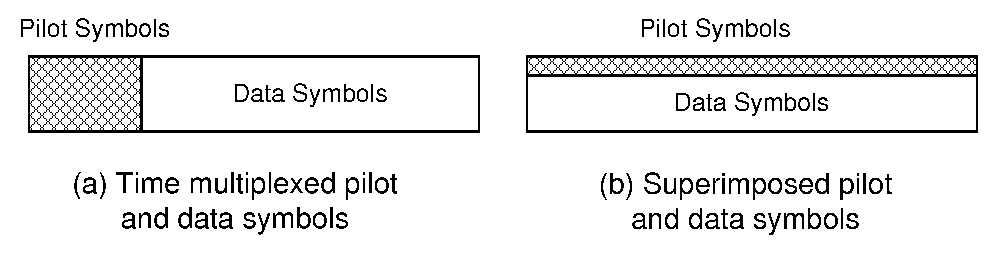
\includegraphics[width=3in, angle=0]{Pilot_Patterns.eps}
\caption{Pilot patterns for channel
estimation.}\label{pilot_pattern} }
\end{figure}

In reality, most MIMO receivers estimate $\bH$ or $\bR_{\bH}$ with
the pilots sent by transmitter at first. Accuracy of the channel
estimation depends on pilot design and placement. There are two
popular pilot patterns, TMP and SIP, receiving much attention for
MIMO channel estimation. They are shown in
Fig.~\ref{pilot_pattern}. TMP is a typical example of orthogonal
pilot design where pilot symbols and data symbols are separated in
time and/or frequency domain, which makes them orthogonal to each
other. With orthogonal pilots, the channel estimation and data
demodulation can be done separately which may lead to simple
receiver design~\cite{Dong02}. SIP does the opposite. In SIP
design, pilots and data nonorthogonally share the same time period
and frequency band. In this case, joint channel
estimation/demodulation and the demodulation with pilot
interference cancellation are among the most popular receiver
design techniques~\cite{Coldrey06}. After channel estimation,
receiver will choose a beamforming vector from a shared MIMO
precoding codebook. This is called channel quantization. And
receiver then feeds back the chosen precoding index(es) to
transmitter(s) instead of actual channel response for the next
transmit precoding. With a MIMO codebook $\bcW$ of the size $2^B$
consisting of $M$-dimensional normalized vectors $\left\{\bw_{1},
..., \bw_{2^{B}}\right\}$, it takes the receiver to feedback $B$
bits for each beam stream. A codebook is usually designed to
quantize channel responses with certain distortion
measures~\cite{Narula98}. This is related to Grassmannian line
packing and the spherical packing on unit sphere
$\bcS_{n}\left(1\right)$~\cite{Love02}, where
$\bcS_{n}(R)=\left\{\bv:\ \left\|\bv\right\|=R\right\}$ denotes
$(n-1)$-sphere of radius $R$. When a codeword $\bw_k$ is chosen to
precode transmit signals for $i$th beam $\bv_{i}$ at the
transmitter side, some degradation will usually happen on the
signals received by receiver because of imperfect channel
estimation and finite-rate feedback. This degradation on received
signals can be expressed by
\begin{equation}\hspace{-0.10in}
\begin{array}{l}
\delta_{i}=\min\limits_{\bw\in\bcW}\left\|\bH(\bv_{i}-\bw)\right\|=\lambda_{i}\left(1-\bv_{i}^{\rm
H}\bw_k\right)-\sum\limits_{j\neq i}\lambda_{j}\bv_{j}^{\rm
H}\bw_{k}
\end{array}\label{delta_i}
\end{equation}
\noindent where $\bv_{i}$ is the ideal precoding vector for the
$i$th eigen-mode. $\delta_{i}$ is known to be one of the major
factors limiting closed-loop MIMO beamforming throughput. There
are two components within $\delta_{i}$. The first term is
\begin{equation}
\begin{array}{rcccl}
\Delta&=&\lambda_{i}\left(1-\bv_{i}^{\rm
H}\bw_k\right)&=&\left(1-\alpha_{i}\right)\lambda_{i}
\end{array},
\end{equation}
\noindent which denotes the degradation of antenna gain with
\begin{equation}
\begin{array}{rcl}
\alpha_{i}&=&\bv_{i}^{\rm H}\bw_k
\end{array}.\label{alpha}
\end{equation}
\noindent The second term is
\begin{equation}
\begin{array}{rcccl}
I_{} & = & \sum\limits_{j\neq i}\lambda_{j}\bv_{j}^{\rm
H}\bw_{k}&=&\sum\limits_{j\neq i}\alpha_{j}\bw_{k}
\end{array}\label{IBI}
\end{equation}
\noindent denoting inter-beam interference (IBI) due to the
correlation between $\bw_{k}$ and other eigen-modes
$\left\{\bv_{j}:\ j\neq i\right\}$. The average received SINR for
the $i$th eigen-mode with the precoding codeword $\bw_{k}$ can be
written by
\begin{equation}
\begin{array}{rcl}
\bar\rho_{i}&=&\mbox{E}_{\bv_{i}\in{\cal
V}_{k}}\left\{\frac{\lambda_{i}\left(\bv_{i}^{\rm
H}\bw_{k}\right)^2P_{i}}{n_{0}^2+ \lambda_{i}\sum\limits_{l\neq
i}^{K}\left(\bv_{i}^{\rm H}\bw_{l}\right)^{2}P_{l}}\right\}\\
&=&\mbox{E}_{\bv_{i}\in{\cal
V}_{k}}\left\{\frac{\alpha_{i}^{2}\rho_{i}}{1+
\lambda_{i}\sum\limits_{l\neq
i}^{K}\frac{\alpha_{l}^{2}}{\lambda_{l}}\rho_{l}}\right\}
\end{array}\label{bar_rho}
\end{equation}
\noindent with $K\leq\mbox{min}\left\{M,\ N\right\}$ the spatial
multiplexity order.

The achievable throughput of MIMO beamforming depends on not only
the chosen precoding vectors $\left\{\bw_{k}:\ k=1,\ 2,\ \ldots,\
K\right\}$ but also the power distribution $\left\{P_{k}:\ k=1,\
2,\ \ldots,\ K\right\}$. There are many power allocation
strategies for assigning transmit power to beams with different
performance metrics. When maximizing throughput is a major
concern, the so-called water-filling strategy can be an option, in
wich each beam's transmit power of each beam satisfies
\begin{equation}
\begin{array}{l}
P_{k}=\left(\mu-\frac{\sigma_{n}^2}{\lambda_{k}}\right)^{+}=
\begin{cases}
\mu-\frac{\sigma_{n}^2}{\lambda_{k}} & \mu-\frac{\sigma_{n}^2}{\lambda_{k}} >0 \\
0 & \mu-\frac{\sigma_{n}^2}{\lambda_{k}} < 0
\end{cases}
\end{array}
\end{equation}
\noindent with $\mu$ chosen so that the total power constraint is
satisfied
\begin{equation}
\begin{array}{rcl}
\sum\limits_{k=1}^{K}P_{k}&=&P
\end{array}.\label{power_constraint}
\end{equation}
\noindent If a delay-limited power allocation strategy is used,
then
\begin{equation}
\begin{array}{rcl}
P_{k}&=&\frac{\mu}{\lambda_{k}}
\end{array}
\end{equation}
with $\mu$ chosen to satisfy (\ref{power_constraint}). It is also
called channel inversion strategy. Another simple but popular
strategy for allocating transmit power is to assign each beam the
average power
\begin{equation}
\begin{array}{rcl}
P_{k}&=&\frac{P}{K}
\end{array}.\label{P_aver}
\end{equation}
In the following sections, we will discuss how the channel
quantization error and imperfect channel estimation affect MIMO
beamforming and MIMO relay network.
\section{Hamming Bound on Channel Quantization}
\begin{figure}
\center{
\includegraphics[width=3.50in, angle=0]{Voronoi_Bounds2.eps}
\caption{(1) Voronoi cell and various bounds. (2) Sphere and
sphere cap.}\label{Voronoi_bound} }
\end{figure}
It is known that the performance of channel quantization depends
on the codebook Voronoi decomposition. If the Voronoi
decomposition is known, the statistic of the $\alpha_i$ defined in
(\ref{alpha}) and the $\bar\rho_{i}$ in (\ref{bar_rho}) can be
calculated. However, the closed-form expression of a general
Voronoi cell boundary is an open-problem even for regular Voronoi
tessellation. This makes it difficult to obtain some insights into
the average SINR and achievable throughput for the MIMO
beamforming with finite-rate feedback. There are two other
well-known open problems related to Voronoi decomposition. The
first one is called disk-covering problem in which, given a unit
disk, the problem is to find the smallest radius for $n$ equal
disks to completely cover the unit disk. The other one is
sphere-packing problem which concerns arrangements of
non-overlapping identical spheres to fill a space. The
relationship between Voronoi cell and the solutions to the
disk-covering problem and sphere-packing problem is illustrated in
Fig.~\ref{Voronoi_bound}. Basically the sphere-packing solution
gives a lower-bound approximation of Voronoi cell and the
disk-covering solution presents an upper-bound approximation of
it. The difference is measured by the parameter called {\em
packing efficiency}, which approaches $1$ when the sphere
dimension becomes large.

Instead of finding the exact boundary for the Voronoi cell
$\bcV_{i}$, we suggest a heuristic approach using Hamming bound
and sphere cap to approximate the actual polytope boundary. It
also is an approximate of the sphere packing solution, in which
all spheres are supposed to be non-overlappedly placed. With our
approach, sphere caps are overlapped with each other in space but
the interior of them has the same area as the Voronoi cell. The
border of this sphere cap is termed Hamming boundary. The
relationship between Hamming boundary and Voronoi cell is shown in
Fig.~\ref{Voronoi_bound}. For an uniform random codebook of size
$2^{B}$ in $M$-dimensional Euclid space, the area of a Voronoi
cell is given by
\begin{equation}
\begin{array}{rcl}
A\left(\bcV_{k}\right)&=&
\frac{2{\pi}^{M}}{2^{B}\Gamma\left(M\right)}
\end{array}\label{V_area}
\end{equation}
\noindent where $\Gamma\left(\ast\right)$ denotes the gamma
function. On the other hand, the area of $(m-1)$-complex sphere
cap $\bcC_{m}^{\rm c}\left(\psi,\ R\right)$ with contact angle
$\psi$ and radius $R$ is
\begin{equation}%\hspace{-0.22in}
\begin{array}{l}
A\left(\bcC_{m}^{\rm c}\left(\psi,\
R\right)\right)=\left[1-\cos^{2(m-1)}\left(\psi\right)\right]S_{m}^{\rm
c}\left(R\right),
\end{array}
\end{equation}
\noindent where ${\bcS}_{m}^{\rm c}\left(R\right)$ denotes a
$M$-dimension complex ball in Euclid space with the radius $R$.
The relationship between ${\bcS}_{m}^{\rm c}\left(R\right)$ and
$\bcC_{m}^{\rm c}\left(\psi,\ R\right)$ can be shown in
Fig.~\ref{Voronoi_bound} and it can be verified that
\begin{equation}
\begin{array}{rcl}
A\left(S_{m}^{c}\left(R\right)\right)&=&A\left(\bcC_{m}^{\rm
c}\left(\pi,\ R\right)\right)
\end{array}.
\end{equation}
%\begin{figure}
%\center{
%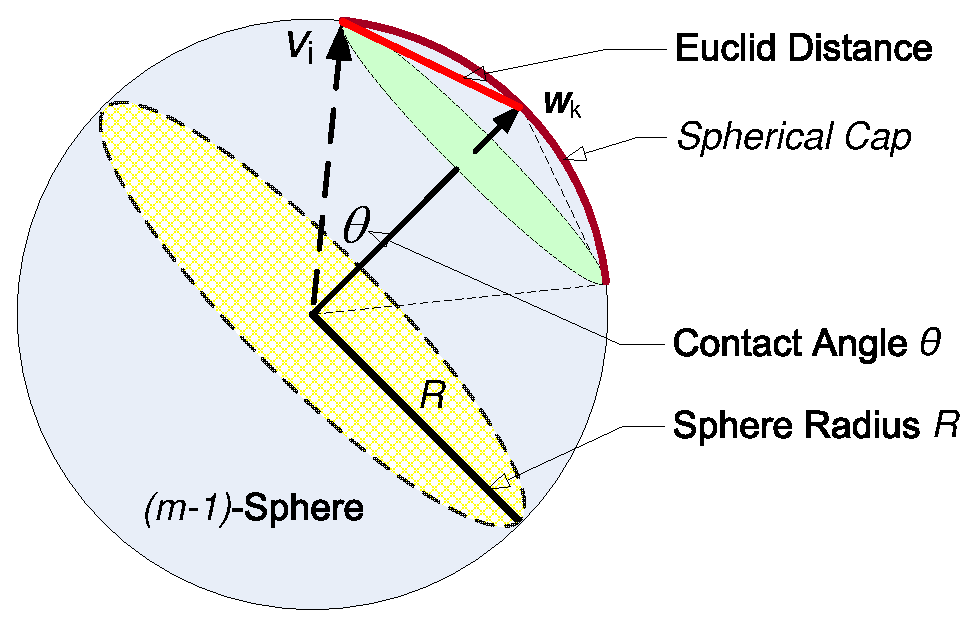
\includegraphics[width=1.80in, angle=0]{Sphere_Cap.eps}
%\caption{Sphere and sphere cap}\label{Sphere_Cap} }
%\end{figure}
\noindent With matching the sum area of the sphere-cap with the
whole sphere area, the boundary of a Voronoi cell can be
approximated by a hypershpere or a closed space curve defined in
the following proposition.
\begin{Prop}\label{approx_bound}(Hamming Boundary) The boundary of the uniform complex Voronoi cell $\bcV_{k}$ can be
approximated by a $(M-1)$-unit complex sphere or a closed complex
space curve.
\begin{equation}\hspace{-0.05in}
\begin{array}{rcl}
\bB\left(\bcV_{k}\right)&\approx& \bcS_{M}^{\rm c}(1)\bigcap \bcL_{M}^{\rm c}(\bw_{k},\ \cos(\theta)) \\
&=&\left\{\bv:\ \left\|\bv\right\|=1,\ \angle\left(\bv,\
\bw_{k}\right)=\theta\right\}\ ,
\end{array}
\end{equation}
\noindent where $\bcL_{M}^{\rm c}\left(\bw_{k},\
\cos(\theta)\right)=\left\{\bv:\ \bv^{\rm
H}\bw_{k}=\cos(\theta)\right\}$ denotes a complex space curve and
$\theta$ is
\begin{equation}%\hspace{-0.00in}
\begin{array}{rcl}
\theta&=&\arccos\left(\alpha_{0}\right)
\end{array}
\end{equation}
\noindent with
\begin{equation}\hspace{-0.00in}
\begin{array}{rcl}
\alpha_{0}&=&\left(\frac{2^B-1}{2^B}\right)^{\frac{1}{2M-2}}
\end{array}.
\end{equation}
\end{Prop}
On the other hand, if the ideal channel precoding vector $\bv_{i}$
is assumed to be a random variable of $M$-dimensional uniform
distribution, the probability density function (PDF)
$\mbox{pr}\left(\alpha\right)$ of $\alpha$ are
\begin{equation}\hspace{-0.10in}
\begin{array}{rcl}
{\rm pr}\left(\alpha\right)&=&\mbox{Prob}\left\{x=\alpha\right\}\\
&=&\begin{cases}
0 & 0\leq \alpha < \alpha_{0} \\
\frac{\left(2M-2\right)\alpha\left(1-\alpha^2\right)^{M-2}}{\left(1-\alpha_{0}^{2}\right)^{M-1}}
& \alpha_{0}\leq\alpha\leq 1
\end{cases}
\end{array}
\end{equation}
\noindent and the cumulated density function (CDF) is
\begin{equation}\hspace{-0.10in}
\begin{array}{rcl}
{\rm Pr}\left(\alpha\right)&=&\mbox{Prob}\left\{x\leq\alpha\right\} \\
&=&
\begin{cases}
0 & 0 \leq\alpha < \alpha_{0} \\
1-\left(\frac{1-\alpha^2}{1-\alpha_{0}^2}\right)^{M-1} &
\alpha_{0}\leq\alpha\leq 1
\end{cases}\ .
\end{array}
\end{equation}
\noindent With the assumption of uniform random codebook and MIMO
channels, the average received SINR $\bar\rho_{i}$ can be
approximated by the following lemma.
\begin{lemma} A heuristic mean of $\rho_{i}$
can be expressed by
\begin{equation}%\hspace{-0.10in}
\begin{array}{rcl}
\bar\rho_{i}&\approx&\frac{\sigma_{\alpha}^{2}\rho_{i}}{1+
\left(\frac{1-\sigma_{\alpha}}{M-1}\right)^{2}\sum\limits_{j\neq
i}\frac{\lambda_{i}}{\lambda_{j}}\rho_{j}}\ ,
\end{array}
\end{equation}
\noindent where $\sigma_{\alpha}$ denotes the standard deviation
of $\alpha$ with
\begin{equation}%\hspace{-0.0in}
\begin{array}{rcccl}
\sigma_{\alpha}^2&=&\mbox{E}\left\{\alpha_{i}^2\right\}&=&\frac{1}{M}+\frac{M-1}{M}\left(\frac{2^B-1}{2^B}\right)^{\frac{1}{M-1}}
\end{array}.\label{sigma_alpha}
\end{equation}
\end{lemma}
\section{Cramer-Rao Bound on Channel Estimat.}
In previous discussions, neither inter-symbol interference (ISI)
nor channel estimation was assumed. In general, the channel
estimation model for frequency-selective block fading channel is
different to (\ref{Direct_MIMO}). In practical channel estimation,
not only the whole channel impulse response but also the pilot
placement should be considered. Considering a $M$-input/$N$-output
MIMO channel with frequency-selective block fading, where the
random channels taps remain constant for some data packets and
change to independent values for the next block, the received
baseband signal can be written by
\begin{equation}\hspace{-0.10in}
\begin{array}{rcl}
\by&=&\left[\begin{matrix}y_{1}(t)&y_{2}(t)&\cdots&y_{N}(t)\end{matrix}\right]^{\rm T}\\
&\hspace{-0.15in}=&\hspace{-0.15in}\left[\begin{matrix}\sum\limits_{m=1}^{M}h_{m,1}(t)\otimes s_m(t)\\ \sum\limits_{m=1}^{M}h_{m,2}(t)\otimes s_m(t)\\ \vdots \\
\sum\limits_{m=1}^{M}h_{m,N}(t)\otimes
s_m(t)\end{matrix}\right]+\left[\begin{matrix}n_{1}(t)\\ n_{2}(t)\\ \vdots\\
n_{N}(t)\end{matrix}\right]=\bS\bh+\bn
\end{array}
\end{equation}
\noindent where $s_m(t)$ denotes the transmitted symbol from the
$m$th antenna, $\bh$ is the stretched channel vector defined by
\begin{equation}\hspace{-0.00in}
\begin{array}{rcl}
\bh&=&\mbox{vec}\left(\left[\mbox{vec}(\bH_{1})\
\mbox{vec}(\bH_{2})\ \ldots\ \mbox{vec}(\bH_{N})\right]\right)
\end{array}
\end{equation}
\noindent with $\bH_{n}=\left[\bh_{n}(0)\ \bh_{n}(1)\ \ldots\
\bh_{n}(L_{c}-1)\right]$, $\bh_{n}(l)=\left[h_{n,1}(l)\
h_{n,2}(l)\ \ldots\ h_{n,M}(l)\right]^{\rm T}$ for $1\leq l \leq
L_{c}$, and
\begin{equation}%\hspace{-0.00in}
\begin{array}{rcl}
\bS&=&\mbox{kron}\left(\left[\bS_{1}\ \bS_{2}\ \ldots\
\bS_{M}\right]^{\rm T},\ \bI\right)
\end{array}
\end{equation}
\noindent with
\begin{equation}%\hspace{-0.10in}
\begin{array}{rcl}
\bS_{k}&=&\left[\begin{matrix}
s_{k}(L)&\cdots&s_{k}(L-L_{c})\\
s_{k}(L-1)&\cdots&s_{k}(L-L_{c}-1)\\
\vdots&\ddots&\vdots\\
s_{k}(1)&\cdots&s_{k}(1-L_{c})
\end{matrix}\right]
\end{array}.\label{S_k}
\end{equation}
\noindent $L_{c}$ is the maximum channel order for all
subchannels. After the channel response vector $\bh$ is estimated,
we can calculate the channel correlation matrix $\bR_{\bH}$ by
\begin{equation}%\hspace{-0.0in}
\begin{array}{rcl}
\hat{\bR}_{\bH}&=&\frac{1}{L_{c}}\sum\limits_{l=1}^{L_{c}}\sum\limits_{n=1}^{N}\hat{\bh}_{n}\left(L_{c}+l\right)\hat{\bh}_{n}^{\rm
H}\left(L_{c}+l\right)
\end{array}.\label{R_h_actual}
\end{equation}

There are many ways putting pilot symbols and data symbols
together for PAT. We focus on two most popular designs: an
{orthogonal design} by {TMP pattern}, and a {non-orthogonal
design} by {SIP pattern}, in this paper.
\subsubsection{Time-Multiplexed Pilots and Data}
The concept of TMP design is to send $Q$ known pilot symbols and
$\left(L-Q\right)$ data symbols consecutively and separately in
time domain. One possible example of TMP is shown in
Fig.~\ref{pilot_pattern}(a), in which the transmitted symbol
$s_{k}(l)$ is
\begin{equation}
\begin{array}{rcl}
s_{k}\left(l\right)&=&
\begin{cases}
s_{pk}(l) & 1 \leq l \leq Q \\
s_{dk}(l-Q) & Q+1\leq l\leq L
\end{cases}
\end{array},\label{TMP_k}
\end{equation}
\noindent where $s_{pk}(t)$, $1\leq t \leq Q$, denotes the pilot
symbols transmitted in power $\sigma_{p}^2$ and $s_{dk}(t)$,
$Q+1\leq t \leq L$, denotes the data symbols transmitted in power
$\sigma_{d}^2$.
\subsubsection{Superimposed Pilots and Data}
In SIP design, data symbols and pilot symbols are simultaneously
sent within one frame of $L$ symbols. This can be shown in
Fig.~\ref{pilot_pattern}(b). In this case, the transmitted symbol
$s_{k}(l)$ becomes
\begin{equation}
\begin{array}{rcl}
s_{k}\left(l\right)&=&\frac{\sigma_{p}}{P}s_{pk}\left(l\right)+\frac{\sigma_{d}}{P}s_{dk}\left(l\right)\
,\ 1\leq l\leq L\ ,
\end{array}\label{SIP_k}
\end{equation}
\noindent with $\sigma_{p}^2+\sigma_{d}^2=P$.

The lower bound to the mean-squared errors (MSE) of unbiased
channel estimates is given by CRLB, which is defined as the
inverse of the Fisher Information Matrix (FIM). If we denotes
$\bvartheta=\left[\bh^{\rm T}\ \bs_{d}^{\rm T}\right]^{\rm T}$,
the complex FIM is given by
\begin{equation}%\hspace{-0.10in}
\begin{array}{rcl}
\mbox{F}\left(\bvartheta\right)&=&\mbox{E}\left\{\left[\frac{\partial\ln\mbox{Pr}\left(\by|\vartheta\right)}{{\partial\vartheta}^{\ast}}\right]\left[\frac{\partial\ln\mbox{Pr}\left(\by|\vartheta\right)}{{\partial\vartheta}^{\ast}}\right]^{\rm
H}\right\}
\end{array}.\label{FIM}
\end{equation}
\noindent With (\ref{FIM}), the MSE of the estimates of
$\bR_{\bh}=\mbox{E}\left\{\bh\bh^{\rm H}\right\}$ is given by
\begin{equation}
\begin{array}{rcl}
\mbox{MSE}\left\{\bR_{\bh}\right\}&=&\sigma_{n}^{2}\left[\mbox{E}\left\{\bS^{\rm
H}\bS\right\}+\rho_{h}^2\bI\right]^{-1}
\end{array},
\end{equation}
\noindent where
$\rho_{h}^{2}=\mbox{E}\left\{\left|\frac{\partial\ln\mbox{Pr}\left(h\right)}{{\partial
h}^{\ast}}\right|^2\right\}$. The CRLB on the channel estimation
therefore is formulated by the following lemma.
\begin{lemma}(Cramer-Rao Lower Bound) For the time-multiplexed pilot and data design defined in
(\ref{TMP_k}), the CRLB of channel estimation is
\begin{equation}
\begin{array}{rcl}
\varepsilon_{h}^{\mbox{\tiny
TMP}}&\geq&\left[\rho_{h}^2+Q\rho_{p}^2+\left(L-Q\right)\rho_{d}^2\right]^{-1}
\end{array}.\label{CRLB_TMP}
\end{equation}
\noindent For the superimposed pilot and data design defined in
(\ref{SIP_k}), the CRLB of channel estimation is
\begin{equation}\
\begin{array}{rcl}
\varepsilon_{h}^{\mbox{\tiny
SIP}}&\geq&\left[\rho_{h}^2+L\left(\rho_{p}^2+\rho_{d}^2\right)\right]^{-1}
\end{array}\label{CRLB_SIP}
\end{equation}
\noindent where $\rho_{p}^2=\frac{\sigma_{p}^2}{\sigma_{n}^2}$
denotes the SNR of received pilot signals and
$\rho_{d}^2=\frac{\sigma_{d}^2}{\sigma_{n}^2}$ denotes the SNR of
received data signals.
\end{lemma}
Now if we look back at (\ref{R_h_actual}) with the assumption that
the channel is constant during estimation, pilots and data are
random and independent to each and an optimal channel estimation
is done by receiver, a heuristic view of the MIMO channel
correlation matrix $\bR_{\bH}$ estimation is
\begin{equation}
\begin{array}{rcccl}
\bDelta_{\bR_{\bH}}&=&\hat{\bR}_{\bH}-\bR_{\bH}&\approx&\frac{\varepsilon_{h}}{\sqrt{L_{c}N}}\bI_{M}
\end{array}.\label{R_h_approx}
\end{equation}
\noindent The eigenvalue estimation error can be approximated by
\begin{equation}%\hspace{-0.1in}
\begin{array}{rcl}
\Delta_{\lambda_{k}}&\approx&\bv_{k}^{\rm
H}\bDelta_{\bR_{\bH}}\bv_{k}-\lambda_{k}\left(\bDelta_{\bv_{k}}^{\rm
H}\bv_{k}+\bv_{k}^{\rm H}\bDelta_{\bv_{k}}\right)
\end{array}\label{lambda_approx}
\end{equation}
\noindent where $\varepsilon_{h}$ denotes the MSE of channel
estimates, which can be either $\varepsilon_{h}^{\mbox{\tiny
TMP}}$ or $\varepsilon_{h}^{\mbox{\tiny SIP}}$. With
(\ref{R_h_approx}) and (\ref{lambda_approx}), it shows that
$\bDelta_{\bR_{\bH}}$ mostly affects the accuracy of the
eigenvalues estimates $\left\{\hat{\lambda}_{k},\ k=1,\ 2,\
\ldots\ K\right\}$ if enough pilots are available. The MSE of
eigenvalue estimates is roughly bounded by
\begin{equation}
\begin{array}{rcl}
\varepsilon_{\lambda}&\gtrsim&\frac{\varepsilon_{h}}{\sqrt{L_{c}N}}
\end{array}.\label{eigenvalue_bound}
\end{equation}
There are two major effects of PAT on MIMO channel throughput. The
first one is that pilot itself will take away channel resources
from data transmission. The second one is that it may affect the
transmit power allocation. If orthogonal pilot pattern is used,
there will be linearly degradation on channel throughput so that
\begin{equation}%\hspace{-0.2in}
\begin{array}{rcl}
\eta^{\mbox{\tiny TMP}}& =&\frac{L-Q}{L}
\sum\limits_{k=1}^{K}\log\left(1+\frac{\hat{\rho}_{i}}{M}\right)
\end{array},\label{spectral_eff_TM}
\end{equation}
\noindent where $\hat{\rho}_{i}$ denotes the suboptimal power
allocation due to channel estimation error, and if superimposed
pilot pattern is employed, the throughput becomes
\begin{equation}%\hspace{-0.2in}
\begin{array}{rcl}
\eta^{\mbox{\tiny
SIP}}&=&\sum\limits_{k=1}^{K}\log\left(1+\frac{\sigma_{d}^{2}}{P}\frac{\hat{\rho}_{i}}{M}\right)
\end{array},\label{spectral_eff_SI}
\end{equation}
\noindent even though the ideal beamforming vectors
$\left\{\bv_{k}:\ k=1,\ 2,\ \ldots,\ K\right\}$ are available.
\section{Multi-Antenna Relay Network}
In order to understand the asymptotic behavior of MIMO beamforming
with channel estimation and quantization, a multi-hop MIMO relay
network with amplify-and-forward transmission in each relay
station is considered. With previous discussions, the follow
conclusion can be reached.
\begin{lemma}
In an amplify-and-forward MIMO relay network where each relay
station has a $M\times N$ MIMO transceiver with spatial
multiplexity order $K$ and each MIMO link is uniform random and
independent to each other with same pilot pattern and codebook,
the end-to-end average throughput for MIMO relay link of the size
$G$ roughly is
\begin{equation}\hspace{-0.10in}
\begin{array}{rcl}
\bar\eta^{\mbox{\tiny
TMP}}&\approx&\frac{L-Q}{L}K\log\left[1+\frac{\rho}{M}\left(\frac{\sigma_{\alpha}^{2}}{1+\frac{(K-1)(1-\sigma_{\alpha})^2\rho}{(M-1)^2}}\right)^{G}\right]
\end{array}\label{RN_TM}
\end{equation}
\noindent if time-multiplexed pilot pattern is used, or
\begin{equation}%\hspace{-0.23in}
\begin{array}{rcl}
\bar\eta^{\mbox{\tiny
SIP}}&\approx&K\log\left[1+\frac{\sigma_{d}^{2}\rho}{PM}\left(\frac{\sigma_{\alpha}^{2}}{1+\frac{(K-1)(1-\sigma_{\alpha})^2\rho}{(M-1)^2}}\right)^{G}\right]
\end{array}\label{RN_SI}
\end{equation}
\noindent if superimposed pilot pattern is used, where
$\rho=\mbox{E}\{\rho_{k}\}$ denotes the average received
beamforing SNR and $\sigma_{\alpha}^{2}$ is defined in
(\ref{sigma_alpha}).
\end{lemma}
\begin{figure}
\center{
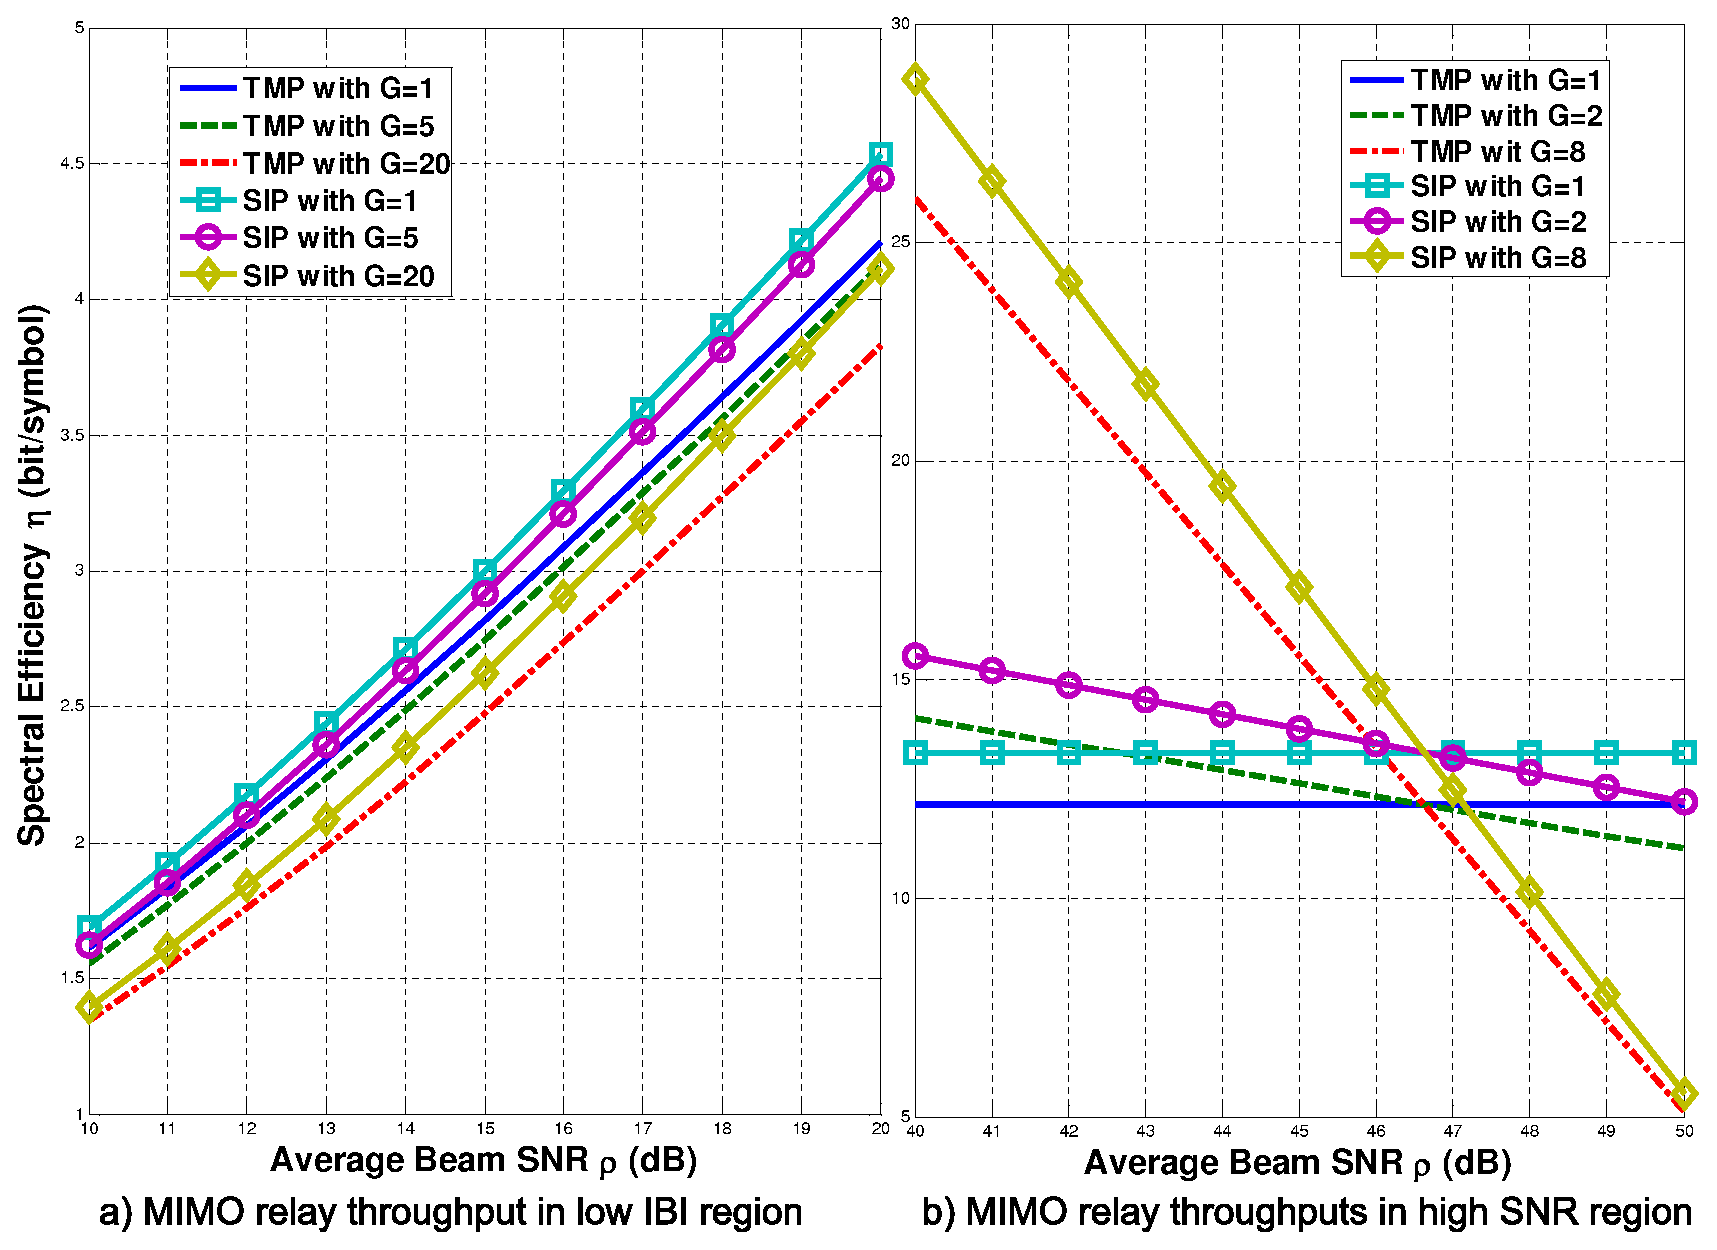
\includegraphics[width=3.2in, angle=0]{MIMO_Relay_Throughput.eps}
\caption{MIMO relay throughput with $M=N=B=4$ and
$\frac{Q}{L}=\frac{\sigma_{p}^{2}}{P}=10\%$
.}\label{MIMO_Relay_Throughput} }
\end{figure}
If the performance of multi-antenna relay network with MISO or
neglectable IBI is considered, the end-to-end throughput with TMP
becomes
\begin{equation}\hspace{-0.15in}
\begin{array}{rcl}
\bar\eta^{\mbox{\tiny
TMP}}&\approx&\frac{(L-Q)K}{L}\log\left[1+\frac{\sigma_{\alpha}^{2G}}{M}\rho\right]
\end{array}\label{RN_TM_MISO}
\end{equation}
\noindent and the end-to-end throughput with SIP is
\begin{equation}\hspace{-0.23in}
\begin{array}{rcl}
\bar\eta^{\mbox{\tiny
SIP}}&\approx&K\log\left[1+\frac{\sigma_{d}^{2}\sigma_{\alpha}^{2G}}{PM}\rho\right]
\end{array}.\label{RN_SI_MISO}
\end{equation}
\noindent They basically are the same as direct MIMO with
additional relay channel degradation factor
$\sigma_{\alpha}^{2G}$. An example of MIMO relay throughput is
shown in Fig.~\ref{MIMO_Relay_Throughput}(a). It shows that SIP is
outperform TMP and the end-to-end throughput of both cases
decreases with more hops. Therefore it may be more efficient to
increase SNR instead of use more hops to increase network
throughput. If the performance of multi-antenna relay network in
high SNR region is concerned, (\ref{RN_TM}) is
\begin{equation}%\hspace{-0.18in}
\begin{array}{rcl}
\bar\eta^{\mbox{\tiny
TMP}}&\approx&\frac{(L-Q)K}{L}\log\left[1+\frac{(M-1)^{G}}{M\rho^{G-1}}\left(\frac{\sigma_{\alpha}}{1-\sigma_{\alpha}}\right)^{2G}\right]
\end{array}\label{RN_TM_high_SNR}
\end{equation}
\noindent and (\ref{RN_SI}) becomes
\begin{equation}%\hspace{-0.23in}
\begin{array}{rcl}
\bar\eta^{\mbox{\tiny
SIP}}&\approx&K\log\left[1+\frac{\sigma_{d}^{2}}{P}\frac{(M-1)^{G}}{M\rho^{G-1}}\left(\frac{\sigma_{\alpha}}{1-\sigma_{\alpha}}\right)^{2G}\right]
\end{array}.\label{RN_SI_high_SNR}
\end{equation}
With (\ref{RN_TM_high_SNR}) and (\ref{RN_SI_high_SNR}), it shows
that the end-to-end throughput of MIMO relay network with channel
estimation and quantization actually will decrease in high SNR
region even though the transmit power of each hop increases. This
can be shown by Fig.~\ref{MIMO_Relay_Throughput}(b), where higher
SNR actually brings down the network throughput and therefore it
may be more efficient to use more hops instead of increase SNR in
each hop to increase network throughput. This means that the
network capacity becomes interference-limited. This is different
to the low-IBI case.
\section{Conclusions}
In this paper, a Hamming boundary for codebook Voronoi
decomposition and the beamforming SINR with finite-rate feedback
are formulated. And the effects of imperfect channel estimation
with time-multiplexed pilot pattern or superimposed pilot pattern
on MIMO beamforming are discussed. Finally the scalability and the
tradeoffs in increasing MIMO relay network throughput with
imperfect channel estimation and quantization are discussed.
\small
\bibliographystyle{unsrt}
\bibliography{Cooperative_Relay}

% that's all folks
\end{document}
